% fig_pipeline.tex  — M1→M3→M4 pipeline block diagram (standalone)
% Compile: pdflatex fig_pipeline
\documentclass[tikz,border=4pt]{standalone}
\usepackage{tikz}
\usetikzlibrary{shapes.geometric,arrows.meta,positioning,fit,backgrounds,calc}

\begin{document}
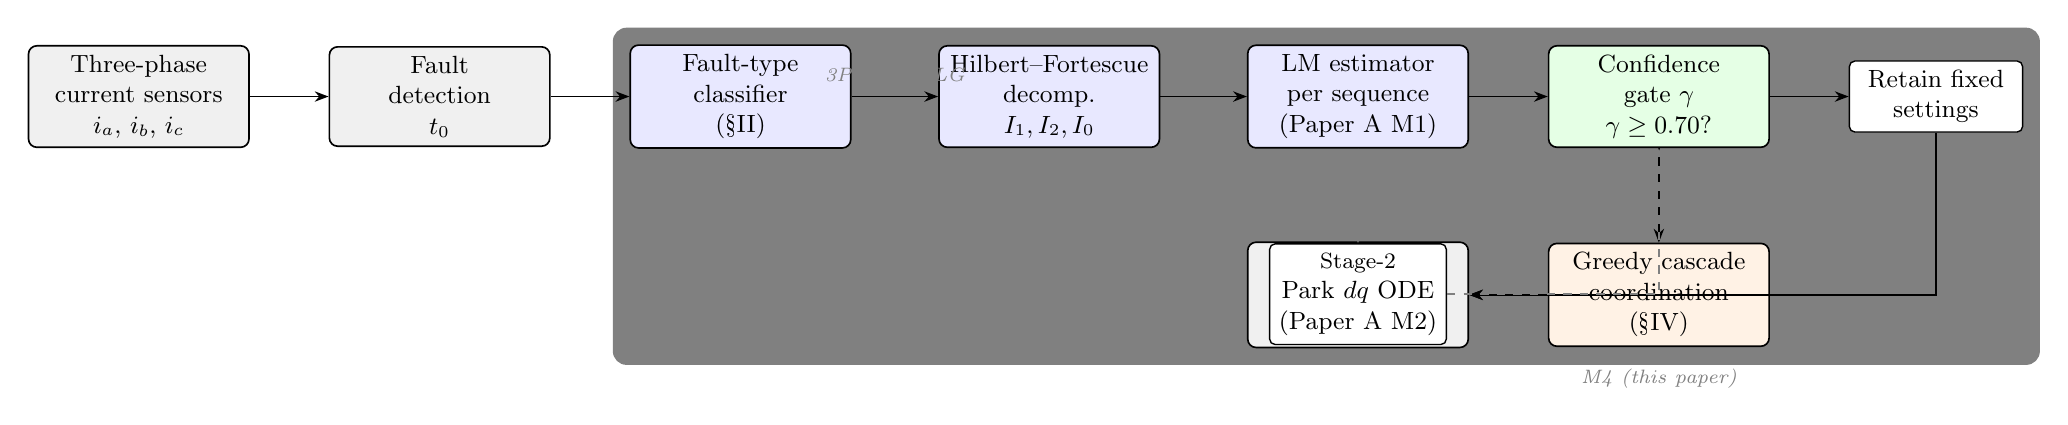
\begin{tikzpicture}[
  font=\small,
  box/.style={draw,rounded corners=3pt,minimum width=2.8cm,minimum height=0.85cm,
              align=center,fill=white,line width=0.6pt},
  smallbox/.style={draw,rounded corners=2pt,minimum width=2.2cm,minimum height=0.75cm,
                   align=center,fill=white,line width=0.5pt},
  graybox/.style={box,fill=gray!12},
  bluebox/.style={box,fill=blue!9},
  greenbox/.style={box,fill=green!10},
  orangebox/.style={box,fill=orange!10},
  arr/.style={-{Stealth[length=5pt]},line width=0.6pt},
  dasharr/.style={-{Stealth[length=4pt]},dashed,line width=0.5pt,gray},
  label/.style={font=\scriptsize\itshape,gray},
]

%% ---- Inputs ----------------------------------------------------------------
\node[graybox] (sensors) {Three-phase\\current sensors\\$i_a,\,i_b,\,i_c$};

%% ---- Fault detection -------------------------------------------------------
\node[graybox, right=1.0cm of sensors] (fdet) {Fault\\detection\\$t_0$};

%% ---- Fault type router -----------------------------------------------------
\node[bluebox, right=1.0cm of fdet] (router) {Fault-type\\classifier\\(§II)};

%% ---- M3 block --------------------------------------------------------------
\node[bluebox, right=1.1cm of router] (hf) {Hilbert–Fortescue\\decomp.\\$I_1,I_2,I_0$};

%% ---- LM per sequence -------------------------------------------------------
\node[bluebox, right=1.1cm of hf] (lm) {LM estimator\\per sequence\\(Paper A M1)};

%% ---- Gate ------------------------------------------------------------------
\node[greenbox, right=1.0cm of lm] (gate) {Confidence\\gate $\gamma$\\$\gamma \geq 0.70$?};

%% ---- M4 coordination -------------------------------------------------------
\node[orangebox, below=1.2cm of gate] (cascade) {Greedy cascade\\coordination\\(§IV)};

%% ---- Relay settings output -------------------------------------------------
\node[graybox, left=1.0cm of cascade] (settings) {Coordinated\\relay settings\\$\{I_{p,k}^*\}$};

%% ---- Fallback (fixed settings) --------------------------------------------
\node[smallbox, right=1.0cm of gate] (fixed) {Retain fixed\\settings};

%% ---- Stage-2 (background, Paper A) ----------------------------------------
\node[smallbox, below=1.2cm of lm] (stage2) {\footnotesize Stage-2\\Park $dq$ ODE\\(Paper A M2)};

%% ---- Arrows: main path -----------------------------------------------------
\draw[arr] (sensors) -- (fdet);
\draw[arr] (fdet)    -- (router);
\draw[arr] (router)  -- node[above,label]{3PH/LL/SLG} (hf);
\draw[arr] (hf)      -- (lm);
\draw[arr] (lm)      -- (gate);

%% ---- Gate branch: accept → cascade → settings
\draw[arr] (gate)    -- node[right,label]{accept} (cascade);
\draw[arr] (cascade) -- (settings);

%% ---- Gate branch: reject → fixed
\draw[arr] (gate)    -- node[above,label]{reject} (fixed);
\draw[arr] (fixed)   |- (settings);

%% ---- Stage-2 dashed reference
\draw[dasharr] (lm) -- node[right,label]{veto} (stage2);
\draw[dasharr] (stage2) -| (gate);

%% ---- Brace labels
\node[below=0.15cm of hf, label] {M3 (this paper)};
\node[below=0.15cm of cascade, label] {M4 (this paper)};
\node[below=0.15cm of lm, label] {M1 (Paper A)};

%% ---- Background shading for "this paper"
\begin{scope}[on background layer]
  \node[fill=blue!5, rounded corners=5pt, inner sep=6pt,
        fit=(router)(hf)(lm)(gate)(cascade)(settings)(fixed),
        label={[label,black]above:This paper (M3 + M4)}] {};
\end{scope}

\end{tikzpicture}
\end{document}
